
\hypertarget{Etat de l'art}{%
\chapter{Etat de l'art}\label{Etat de l'art}}
\section{Etat de l'art}
\label{Etat de l'art}

Quand je suis arrivé dans l'équipe plusieurs solutions basés sur les réseaux de neurones avaient déjà été explorés par mes tuteurs.
La première partie sera donc consacrée à la découverte théorique des réseaux de neurones artificiels et a la convolution.

\subsection{Fonctionnement des réseaux de neurones}
La plupart de mes connaissances sur le sujet vient des présentations que m'ont faites les membres du groupe \textbf{SpikeTrain}, ainsi que d'un livre, co-écrit par le Pr. Paugam Moisy~\cite{naturalHandbook}.
En voici donc un rapide résumé.

\subsubsection{Neurone artificiel}
\label{neuroneClassique}
Tout d'abord avant de parler de réseaux de neurone à spike il serait de bon ton d'expliquer le principe du réseau de neurone classique, explication qui commencera par expliquer le
le principe du neurone unique.

Un neurone artificiel est pourvu d'un certain nombre d'\textbf{entrées}. Dans le cas des neurones classiques, ces entrées sont des nombres réels. Le neurone calculera, en fonction de ces entrées, une unique valeur en \textbf{sortie}.
Détaillons la façon dont ces calculs sont effectués:

Chacune de ces entrées circule sur une connection, laquelle est caractérisée par un \textbf{poids} qui définit l'importance de l'entrée pour le neurone.

Le neurone calcule dans un premier temps la somme de ses entrées, pondérée par leurs poids respectifs, à laquel vient s'ajouter un \textbf{biais} spécifique à chaque neurone (cf. equation~\ref{sommePonderee}).

\begin{equation}
\label{sommePonderee}
y = \sum_{i}^{n} w_i \times x_i + b
\end{equation}

Le résultat de cette somme passe alors dans une \textbf{fonction d'activation} qui permet d'introduire une non-linéarité dans les calculs. La sortie $s$ du neurone est donc calculée conformément à l'équation~\ref{calcNeurone}

\begin{equation}
\label{calcNeurone}
s = f(\sum_{s=0}^{n_{x}} x_{n}w_{n} + b)
\end{equation}

Un schéma reprenant ces explications est présenté dans la figure~\ref{neuroneSeul} :

\begin{figure}[h]
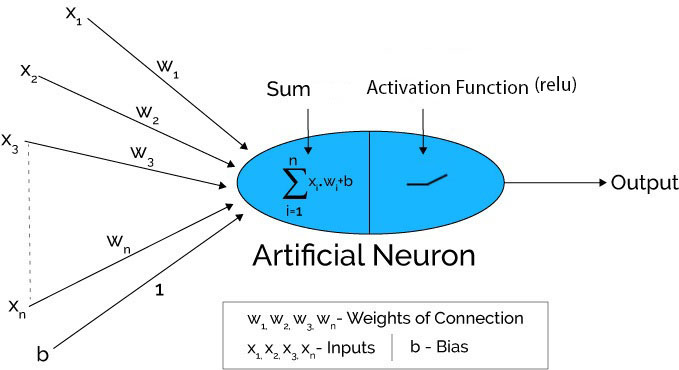
\includegraphics[width=16.5cm]{./images/image2.jpg}
\label{neuroneSeul}
\caption{Fonctionnement d'un neurone seul}
\end{figure}

Notre apprentissage ce fera en modifiant les poids de ses différentes
connexion (et le biais) de façon à obtenir une sortie proche de celle voulu.\newline

\subsubsection{Réseaux de neurones}
\label{Réseaux de neurones}

Les neurones présentés précédemment prennent tout leur intérêt lorsqu'ils sont utilisés en groupes, dans des \textbf{réseaux de neurones}.

Le premier de ces réseaux, encore utilisé de nos jours, est appelé \textbf{perceptron}.
Le principe du perceptron n'est pas nouveau et date des années 1960.

Dans ces réseaux, les neurones sont organisés en \textbf{couches}.
La première couche correspond à celle qui permettra d'introduire des informations dans le réseau (comme la rétine par exemple). Elle est nommé \textbf{couche d'entrée}
La dernière couche permettra de lire les décisions du réseau. Elle est appelée \textbf{couche de sortie}. Dans les applications classiques, à chaque neurone de la couche de sortie correspond une décision possible et le neurone qui est le plus activé sur la couche de sortie l'emporte.
Entre ces couches, on trouve souvent un nombre variable de couches intermédiaires appelées \textbf{couches cachées}.

Entre deux couches, on établit le plus souvent un schéma de connexion que nous pouvons qualifier de \textit{full connected}, c-a-d que chaque neurone d'une couche est connecté avec chaque neurone de la couche suivante.Nous allons encore une fois, pour le bien de ce rapport, ne pas épiloguer sur les autres types de connexions existantes.\newline

Nous allons, pour cette partie encore, utiliser une figure (\ref{reseauClassique}) pour illustrer nos propos:

\begin{figure}[h]
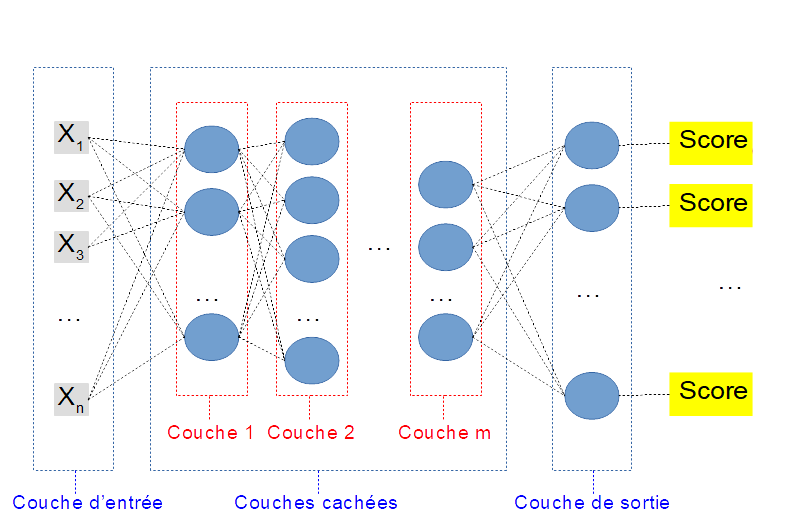
\includegraphics[width=16.5cm]{./images/multicouche.png}
\caption{réseau de neurones classique en couches}
\label{reseauClassique}
\end{figure}


\subsection{la convolution}
\label{la convolution}




\section{Etat des lieux a mon arrive}
\label{Etat des lieux à mon arrivé}

Quand j'ai commencé mon stage mes tuteurs avaient déjà commencé le challenge depuis un moment déjà c'est pourquoi j'ai du dans un premier temps me mettre à jours sur le challenge et ce qu'ils avaient fais.






De plus ceux ci rencontraient un probléme récurant qui était une grande disparité dans leurs résultats sur la base labelisée et leurs résultats sur la base non labelisée.
C'est entre autre pour cette raison que j'ai été chargé de m'occuper de l'analyse des données


\chapter{Analyse des données}\label{Analyse des données}}
\hypertarget{analysedesdonnees}{%
\section{Analyse des données}

\subsection{La base d'apprentissage}

\begin{figure}[!h]
\centering
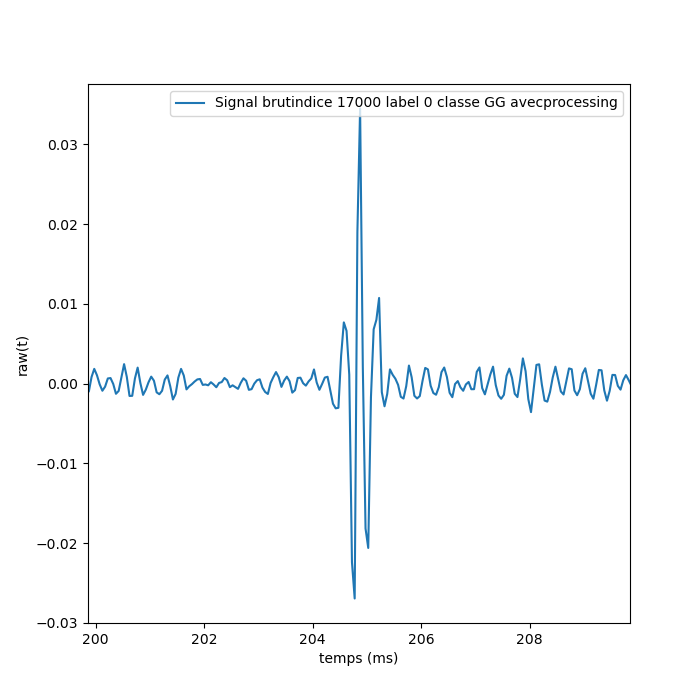
\includegraphics[width=10cm]{./images/indice17000Spectro1Dlabel0classeGGavecprocessingaveczoom.png}
\caption{test}
\end{figure}

\begin{figure}[!h]
\centering
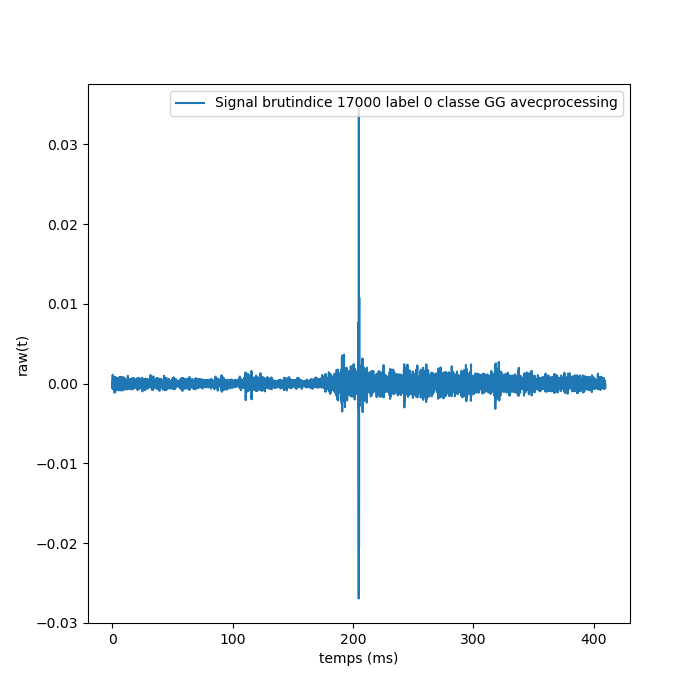
\includegraphics[width=10cm]{./images/indice17000Spectro1Dlabel0classeGGavecprocessingsanszoom.png}
\caption{test}
\end{figure}

\begin{figure}[!h]
\centering
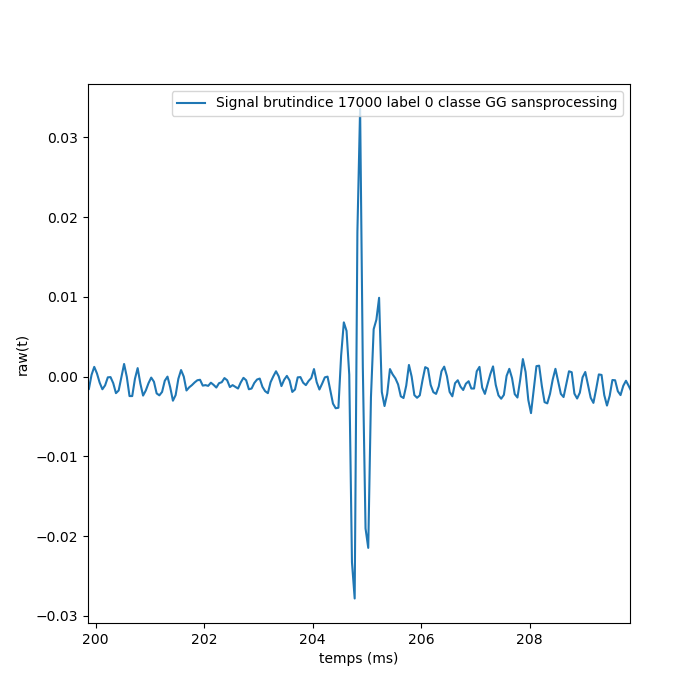
\includegraphics[width=10cm]{./images/indice17000Spectro1Dlabel0classeGGsansprocessingaveczoom.png}
\caption{test}
\end{figure}

\begin{figure}[!h]
\centering
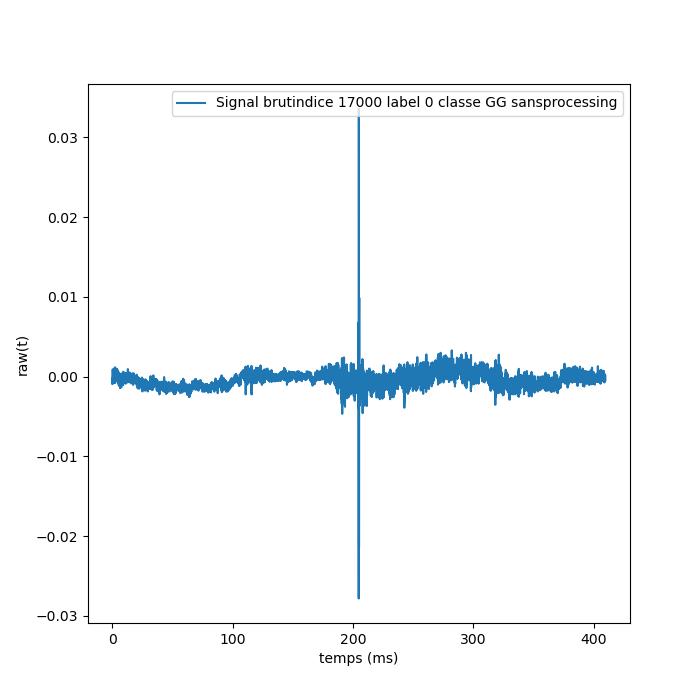
\includegraphics[width=10cm]{./images/indice17000Spectro1Dlabel0classeGGsansprocessingsanszoom.png}
\caption{test}
\end{figure}

\subsection{La base de test}

\subsection{Traitement du signal}

\subsection{Data augmentation}


\subsection{difficultés rencontrées}





\chapter{Le travail a distance}\label{Le travail à distance}}
\section{Le travail a distance}


Comme vous le savez certainement durant cette année 2020 nous avons été touchés par la crise du coronavirus qui nous a conduit a être confinés nous forçant a travailler uniquement a distance.

Ces circonstances très particuliéres ont grandement affecté notre travail particulérement au début ou nous avons du régler de nombreux problémes techniques et organisationels. Cependant en nous forçant a nous adapter a ces nouvelles conditions, cette crise nous a permis de grandement augmenter nos competances en "télétravail".

Ainsi malgrés des débuts léthargiques nous avons mis en place une "routine de travail" qui était la suivante :
-Des visio-conférences quotidiennes nous permettant d'organiser et de synchroniser notre travail
-Un groupe whatsap dédié a mon stage afin de communiquer le plus efficacement possible
-Un Github privé dédié afin de partager l'ensemble du projet
-Un partage régulier de google collab via google drive



\subsection{Outils utilisés}

\subsection{Présentation de GitHub}

\begin{figure}[h]
  \begin{center}
  
\includegraphics[width=5cm]{./images/github.jpg}
  \end{center}
\end{figure}

Nous pouvons définir GitHub comme une plateforme de développement de projet in formatique en groupe. Elle s'implifie grandement le développement de projets. Elle permet de versioner ses programme et d'y apporter des modification en temps réel à plusieurs.

\subsubsection{Pourquoi Github}
Car celà permet une certaine synergie avec nos autres outils que nou verrons plus tard. Cette plateforme permet une facilité de développement de par sa fonctionnalité de versionnage de notre code à chaque changement ce qui permet une mise à jour dynamique ainsi que une relative facilitée a retourner à un état entérieur de notre programme ce qui permet une faciliter de débogage.Nous pouvons d'ailleur dire que ce rappport est entreposer sur Github et qu'il peut être récupérer facilement.Cette plateforme est aussi très connu dans le monde de la programmation ce qui sera utile pour notre future professionnel.

\subsection{Présentation de Google Colab}

\begin{figure}[h]
\begin{center}

\includegraphics[width=5cm]{./images/Colab_logo.png}
\end{center}
\end{figure}

Colab peut-être défini comme étant une plateforme d'éxécution pour notre code
il permet du fait que ce soit la puissance de calcul d'ordinateur géré par Google une vitesse d'exécution ainsi qu'une vitesse de téléchargement de base de données supérieur à celle qui nous est disponible en local.

\subsubsection{Pourquoi Colab}
En premier lieu pour la faciliter d'exéccution du code car ce n'est pas en local ce qui permet une exécution quasi immédiate du code sans aucune installation.Il est aussi facile de mettre sur github du code produit avec colab car c'est deux plateforme sont liées. Il permet de par l'utilisation du format Jupyter de mélanger code et texte (peu aussi comporter des images) dans notre notebook.

Voilà un exmple d'exécution avec colab:

\begin{figure}[h]
\begin{center}
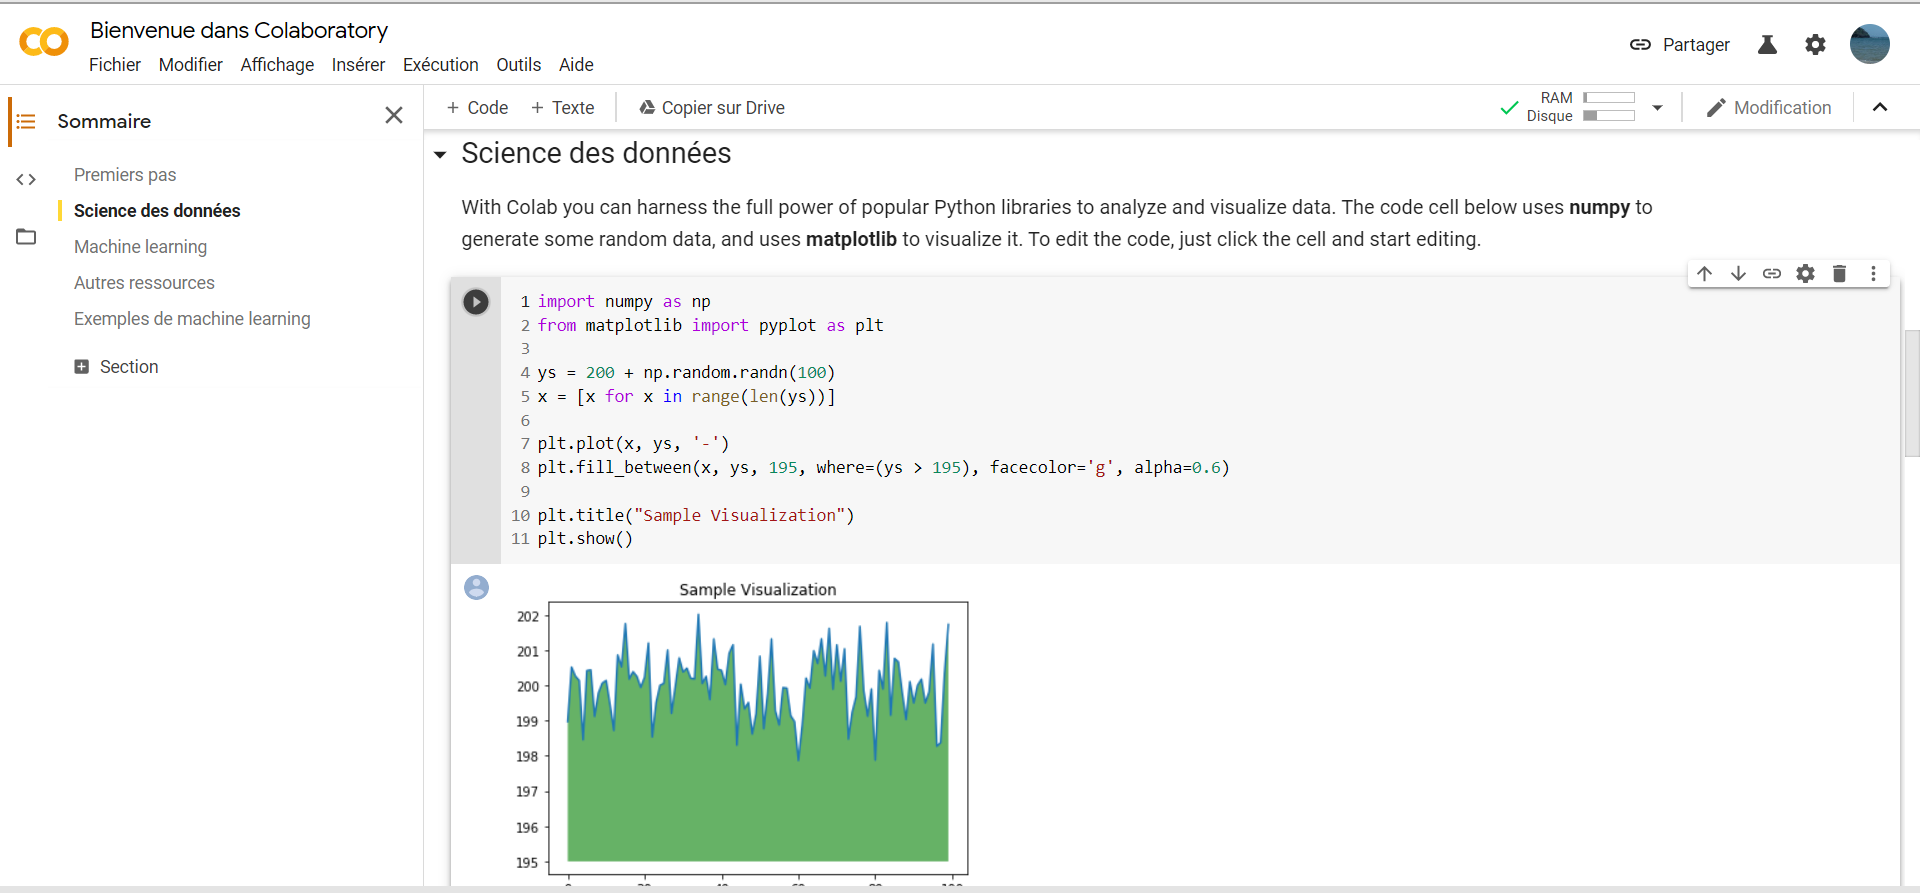
\includegraphics[width=15cm]{./images/Cap_colab.PNG}
\caption{Nous avons ici un exemple de code exécuté avec colab.}
\end{center}
\end{figure}


\subsection{Présentation de LaTex}

\begin{figure}[h]
  \begin{center}

\includegraphics[width=5cm]{./images/Latex.png}
\end{center}
\end{figure}

Nous pouvons dire que LaTex est un langage de traitement de texte tel que le markdown qui permet de mettre en forme notre texte de manière \"scientifique\" cela veut dire que. LaTex permet une faciliter d'écriture des équations et de toutes les écriture mathématiques.Permet de par ses nombreux package une quasi-infinité de possibilitées.
